\chapter{Conclusion and Suggestion}
\section{Conclusion}
% Chapter 6
% Conclusion
% Valar Morghulis.
% – George R. R. Martin,
% A Song of Ice and Fire


We have successfully build an application that can be used to conduct prospective memory error experiment.
The application support configurable setting which allows researcher to change experiment properties and to conduct
an experiment using a large sample. The application has been made publicly available on the github repository.

By using the aplication three studies has been succesfully conducted.
This study is based on conduct Carlson's studies. From the result of the studies,
we can draw a three conclusion. Firstly, the participant experiences prospective memory error while using the smartphone.
Secondly, the increasing number of intention make people more likely to experience prospective memory error (intentional loads matter).
Lastly, Moving through event boundary mentally or physically \textit{probably} increase the likeliness of prospective memory failure.
These first two results support the result of Carlson's experiment. While the last one
contradict their result.

% We have presented the
% Track
% application and associated software components as
% a solution to MacLean’s requirement for the development of a custom Android app
% which  would  enable  her  carry  out  an  emotion  management  study  with  adolescents
% at-risk  of  psychosis.   Furthermore,  we  have  implemented  the  application  in  such  a
% way  that  it  can  be  configured  for  use  in  custom  ESM  studies  by  other  psychology
% researchers,  with support for configuration both at the study and survey level.   The
% application also includes an in-app feedback module allowing users to track their emo-
% tions as they progress through the sampling period.
% Track
% has been made publicly
% available on the Google Play store to make it easier for MacLean to distribute to her
% participants, and also supports a non-participant mode for users who want to use the
% app to personally track their daily emotions and activities.
% All  software  components  have  been  made  available  as  part  of  an  open-source
% project on GitHub, and we have also highlighted suggestions for future work which
% can  be  carried  out  to  improve  the  overall  solution.   This  includes  the  implementa-
% tion of a forms-based survey builder to provide a user interface for psychology re-
% searchers to build custom questionnaires with, and extending the current API to enable
% the
% Track
% application to also support a completely configurable feedback module. Once
% MacLean’s study is underway, it would also be interesting to carry out a compliance
% comparison study to determine whether participants making use of the application did
% or did not show a higher compliance rate as compared to others using the paper-based
% version.


\section{Future suggestion}

\subsection{Experiment application suggestion}

To make a more dynamic and ready to public use, the experiment application still have a lot of features that need to be implemented.
The application should have more user friendly setting so the experimenter can easily set the experiment properties and upload the input file.
On the analysis of the data, it's quite hard to analyze the questions and answer object because there is no field that shows the order of the question, so
 the field that shows the order of the question should be made.

To have better understanding about the event boundary, the question and the answer page presented should be more complex and require
the participant to search the answer by clicking multiple links on the answer page.
Moreover, The application should able to track the movement of the participant so the further analysis can be made on the effect of physical movement
on the failure of prospective memory.


\subsection{Experiment design suggestion}
On the future, I hope that the experiment can be conducted on the bigger sample of participants, and the smartphone of the experiment can be the
personal smartphone of the participant. This will make the participant more comfortable to do the experiment and the failure of prospective memory
phenomena can be analyzed more practically.
I think rather than using a smartphone, the experiment can be conducted by using virtual reality (VR) so the immersion that the participant experience
will be much higher and the study can be more precise on investigating the prospective memory error in everyday life.

\subsection{Futher investigation}
I also suggest that there is a further investigation on the intention and how it stored on the memory. Also, there should be a investigation
whether an intention that is correlated with each other, for example buying a jeans and shirt, can makes people easier to remember than
buying a cake and a shirt. The motivation to formed the intention should also be investigated, such as giving the participant reward if they do
a better prospective memory task.
% \begin{appendices}
% \chapter{Some Appendix}
% 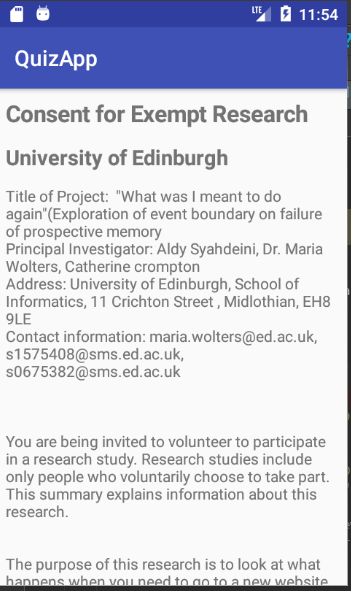
\includegraphics[scale=0.5]{INTRO}
% \end{appendices}


% \begin{figure*}
% \begin{multicols}{3}
% \centering
%     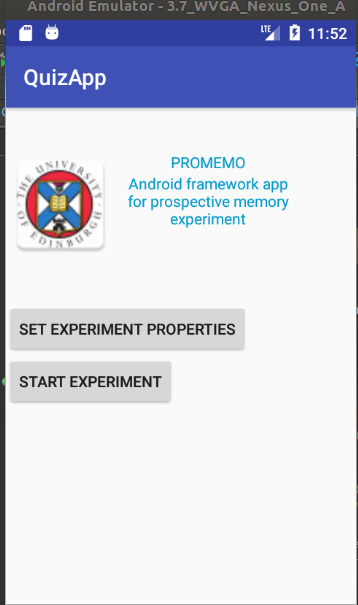
\includegraphics[scale=0.37]{FE_1}
% \caption{}
% \label{fig:ASAs}\par
% 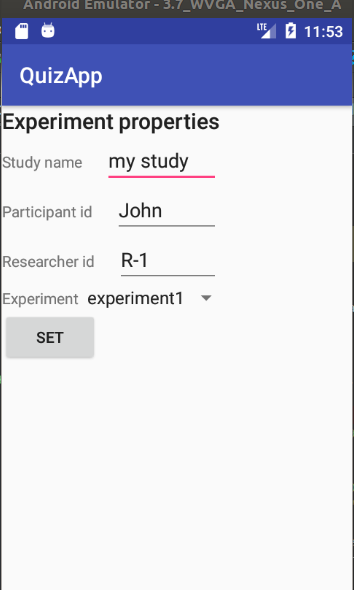
\includegraphics[scale=0.37]{FE_set_properties}
% \caption{Quiz flowchart}
% \label{fig:quiz_flASAsowchart}\par
% 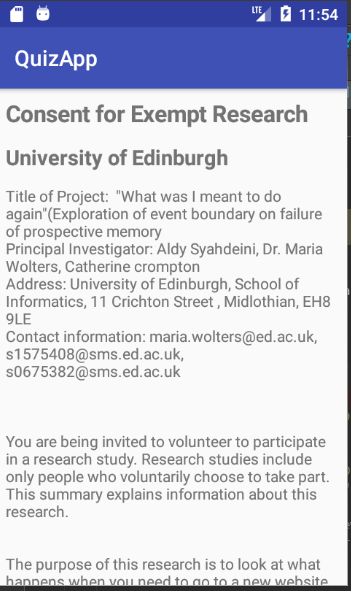
\includegraphics[scale=0.37]{INTRO}
% \caption{Quiz flowchart}
% \label{fig:asdasd}\par
% \centering
%     \end{multicols}
% \end{figure*}
